\chapter{组合卷积结构:自适应卷积模块}
\label{cha:sap}

\section{引言}
\label{sec:sap:introduction}
在过去的十几年时间里,卷积神经网络在计算机视觉领域取得了巨大的成功。尤其是在物体识别、检测和分割等任务中,卷积神经网络的识别与检测精度远远超过了传统方法,连续打破了多个公开数据集的记录。通过卷积神经网络学习到的特征,比传统人工设计的特征(例如SIFT~\cite{lowe1999object, ke2004pca,ke2004pca}特征和HOG~\cite{dalal2005histograms}特征等)更为有效, 这使得卷积神经网络在计算机视觉领域的多项任务中均取得了重大的研究突破。

视觉物体识别是计算机视觉领域一个经典的问题。很多著名的卷积神经网络模型,例如盗梦空间网络结构Inception~\cite{szegedy2014going,szegedy2015rethinking,szegedy2016inception},最大化输出单元Maxout~\cite{goodfellow2013maxout},残差网络ResNet~\cite{he2015deep},和网络中的网络NIN(Network in Network)~\cite{DBLP:journals/corr/LinCY13}被学者们相继提出,用以提升网络的识别精度。但是,对于一个新的问题,设计并实现一个有效的网络模型仍然是一项困难的工作。例如,网络深度的选择就是一个很常见,却又很难回答的问题。VGG~\cite{simonyan2014very} 和GoogLeNet~\cite{szegedy2014going}的成功说明,更深的网络可以提高网络的识别性能。但是,仍然有一些实验~\cite{he2015deep} 表明,在深度持续加深的过程中,网络的测试精度将会趋于饱和甚至下降。另一个需要面对的难题是感受野大小的选择问题,VGG~\cite{simonyan2014very}的成功说明采用 $3\times3$ 的感受野是一个有效的策略,更大的感受野可以通过多个 $3\times3$ 感受野大小的卷积堆叠来实现。但是Inception~\cite{szegedy2014going,szegedy2015rethinking,szegedy2016inception}通过采用具有不同感受野的多个分支来进一步提高网络的识别能力。与之类似地,ResNet~\cite{he2015deep}采用短连接的方式来改变网络的感受野大小,同样也可以进一步提高网络的识别能力。

借鉴上述网络结构的特点与优势,本章提出了一种组合卷积结构:自适应模块(Self-Adaptive Module,SAM),来简化复杂网络的设计过程。结合多种有效卷积神经网络模型的优势,SAM被设计成一个通用的卷积模块,使用组合卷积结构可以简化深层卷积神经网络的设计过程。通过多个组合卷积结构的简单堆叠,来实现复杂深层网络的特征提取与泛化能力。为了实现这样的目标,SAM必须具有自适应的能力。换句话说,SAM采用端到端学习的方式,根据网络不同深度的功能需求,学习成合适的结构。这样,一个大规模的深度卷积神经网络就可以通过SAM层的简单堆叠来设计实现。本章提出的SAM结构以盗梦空间网络结构Inception~\cite{szegedy2014going,szegedy2015rethinking,szegedy2016inception}为基础框架,包括四条特征提取分支和一个特征选择器。四条分支中包含两条卷积分支,它们具有不同的深度和感受野;一条最大化输出单元Maxout\cite{goodfellow2013maxout}分支,用于增强SAM的非线性拟合与逼近能力;一条残差~\cite{he2015deep}分支,可以加快SAM的收敛速度。选择器~\cite{DBLP:journals/corr/LinCY13}通过监督学习的方式对特征进行选择,同时在一定程度上起到特征压缩,降低网络计算复杂度的目的。

我们在多个物体识别的数据集上对SAM进行了实验验证,在CIFAR-10~\cite{krizhevsky2009learning},CIFAR-100~\cite{krizhevsky2009learning},MNIST~\cite{lecun1998gradient}和SVHN~\cite{netzer2011reading}四个公开数据集上均取得了优越的性能。本章其余内容组织如下:第~\ref{sec:sap:ralate}节简要综述了相关工作;第~\ref{sec:sap:review}节回顾了SAM直接继承的四个网络的特点与优势;第~\ref{sec:sap:model}节详细阐述了SAM的结构与特点;第~\ref{sec:sap:experiment}节对SAM进行了实验验证与对比分析;第~\ref{sec:sap:conclusion}节总结了本章的主要内容。


\section{相关工作}
\label{sec:sap:ralate}

据我们所知,最早的卷积神经网络模型是1975年Fukushima~\cite{fukushima1982neocognitron} 提出的认知机(Cognitron)~\cite{fukushima1975cognitron} 和神经认知机(Neocognitron)~\cite{fukushima1980neocognitron}模型。在他的重要论文~\cite{fukushima1982neocognitron} 中,提出了包含卷积、感受野~\cite{hubel1959receptive, hubel1962receptive}和池化等概念的神经认知机计算模型。1989年,LeCun~\cite{le1988theoretical, lecun1989backpropagation, le1990handwritten}将误差的反向传播(back-propagation)引入神经认知机模型,并且成功应用于手写体数字识别数据集MNIST上,奠定了现代卷积神经网络的计算框架。

2012年,Krizhevsky等人~\cite{krizhevsky2012imagenet}采用卷积神经网络,借助于高性能的GPU并行计算能力,在2012年ImageNet大规模视觉识别比赛(ImageNet Large Scale Visual Recognition Competition,ILSVRC)中夺冠,掀起了卷积神经网络的研究热潮。此后,越来越多的深度卷积神经网络模型被应用于视觉物体识别任务,例如OverFeat~\cite{sermanet2013overfeat},VGG~\cite{simonyan2014very},GoogLeNet~\cite{szegedy2014going,szegedy2015rethinking,szegedy2016inception} 和ResNet~\cite{he2015deep}等。

在CIFAR-10~\cite{krizhevsky2009learning},CIFAR-100~\cite{krizhevsky2009learning},MNIST~\cite{lecun1998gradient}和SVHN~\cite{netzer2011reading} 四个个数据集上,同样是很多学者的研究重点。Goodfellow等人~\cite{goodfellow2013maxout}提出了一种新的激活函数形式Maxout。Maxout具有很强的特征拟合能力,如果隐层具有足够多的神经元,理论上Maxout可以逼近任意复杂的非线性函数。Lin等人~\cite{DBLP:journals/corr/LinCY13}采用网络中的网络(Network in Network,NIN)来提高模型局部感受野范围内的特征非线性拟合能力,同时,Lin提出了全局池化来提取固定长度的特征,用于视觉物体分类任务,在一定程度上起到防止过拟合的效果。Wan等人~\cite{wan2013regularization}提出了DropConnect方法,该方法是Dropout方法的一种推广,用于对全连接层进行正则化。Zeiler and Fergus~\cite{zeiler2013stochastic}对池化方法进行了改进,提出了随机池化,在池化区域内根据多项式分布进行特征的随机采样。Stollenga等人~\cite{stollenga2014deep} 将注意力模型引入卷积神经网络的卷积核,提出了dasNet。Lee等人~\cite{lee2014deeply}同时对网络的隐层和输出层进行监督学习,提出了深度监督网络(Deeply-Supervised Nets,DSN)。Liang和Hu~\cite{liang2015recurrent}提出递归卷积神经网络RCNN,通过在卷积层引入递归连接,增大局部区域内卷积的感受野范围,结合图像上下文特征来提高网络的物体识别能力。Srivastava等人~\cite{srivastava2015training}将卷积网络逐层特征提取的过程当做信息流动,在网络结构中引入短连接,使特征以信息的形式通过短连接高速跨层流动,加快网络的收敛速度,提出了Highway网络结构。He等人\cite{he2015deep}提出了残差模型,设计并实现了ResNet网络,在CIFAR-10,ILSVRC 2015~\cite{everingham2010pascal}和COCO~\cite{lin2014microsoft}等数据集上均取得了巨大的成功。

对于视觉物体识别任务,在网络结构上也陆续出现了多种改进方法。1989年,LeCun等人~\cite{lecun1989backpropagation,le1990handwritten}将误差反向传播算法引入到神经认知机模型中,提出了著名的LeNet-5网络,奠定了现代卷积神经网络的计算框架。2012年,Krizhevsky等人~\cite{krizhevsky2012imagenet}提出了一个与LeNet-5类似,但结构更深的卷积神经网络模型AlexNet,借助于高性能的GPU并行计算能力,在2012年ImageNet大规模视觉识别比赛(ImageNet Large Scale Visual Recognition Competition,ILSVRC)中一举夺冠,掀起了卷积神经网络的研究热潮。
2014年,Zeiler~\cite{zeiler2014visualizing}提出了一种网络中间层特征的可视化方法,用来探索卷积神经网络的工作原理,结合网络可视化结果提出了ZFNet。同年,Simonyan~\cite{simonyan2014very}和Szegedy~\cite{szegedy2014going}分别提出了VGGNet和GooLeNet,在2014年ImageNet比赛中分别取得了冠亚军的好成绩。其中GooLeNet提出的Inception结构在增加特征表达能力的同时减少了计算量。
2015年,随着批正则化方法BN~\cite{ioffe2015batch}的提出,Inception过渡到了第二个版本。
同年,Szegedy借鉴当时最新的网络设计原则,采用2个 $3\times3$ 的卷积核代替原来 $5\times5$ 的卷积核,进一步减少了模型参数和计算量,提出了Inception的第三个版本v3。2016年,Szegedy~\cite{szegedy2016inception}将Inception和残差网络ResNet~\cite{he2015deep}相结合,提出了Inception-v4结构,进一步提高了ImageNet数据集的识别率。2017年,Huang等人~\cite{huang2016densely}借鉴残差网络和Inception的思想,提出了一个全新的网络模型DenseNet,可以进一步减弱梯度消失问题。

\section{重要网络结构的简要回顾}
\label{sec:sap:review}

本节简要回顾了四种用于视觉物体识别的卷积网络模型,分别是盗梦空间网络结构Inception~\cite{szegedy2014going,szegedy2015rethinking,szegedy2016inception},最大化输出单元Maxout~\cite{goodfellow2013maxout},残差网络ResNet~\cite{he2015deep},和网络中的网络NIN~\cite{DBLP:journals/corr/LinCY13}。SAM继承了这四个模型结构的主要特点与优势,用于简化复杂卷积网络的设计难题。

\begin{figure*}[t]
\centering
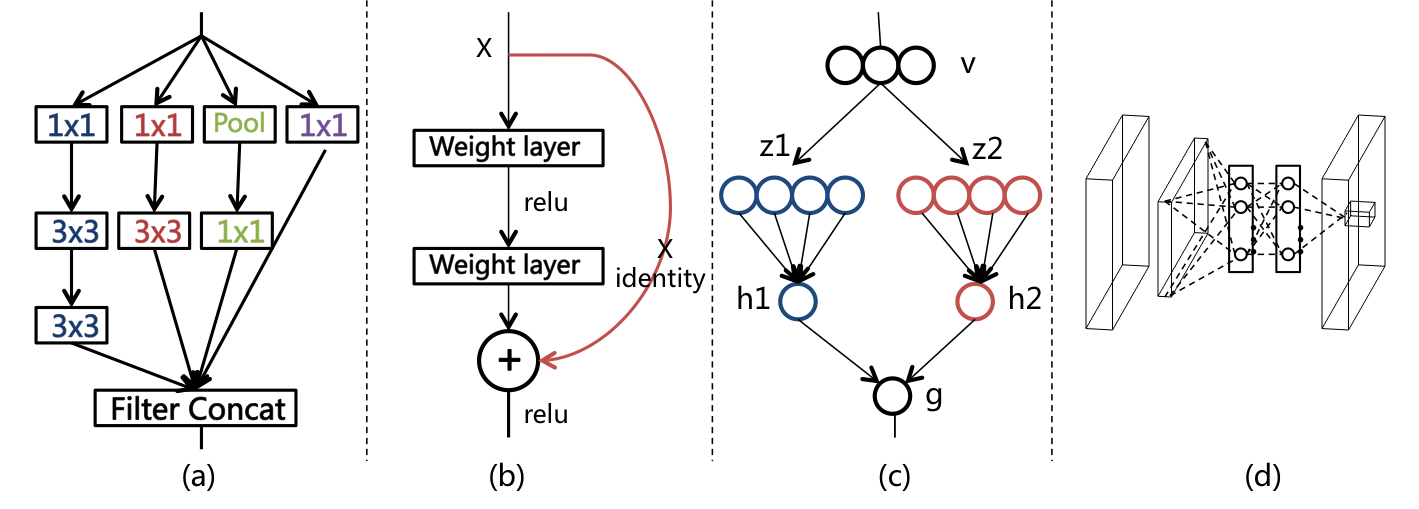
\includegraphics[width=1.0\linewidth]{sam_review.png}
\caption{重要网络结构的简要回顾. (a) Inception, (b) ResNet, (c) Maxout, (d) NIN}
\label{fig:sam_review}
\end{figure*}

\subsection{Inception}
\label{sec:sap:review:inception}

GooLeNet具有4个版本~\cite{szegedy2014going,ioffe2015batch,szegedy2015rethinking,szegedy2016inception},其中最为核心结构就是盗梦空间Inception结构。虽然Inception在多个版本的迭代中有所调整,但仍保持着最初的设计初衷。自AlexNet和VGG取得成功以后,大家普遍认识到加大网络的深度和宽度,可以有效提高网络的识别能力。但是这样做会带来两个问题:过拟合和计算量的增加。Inception的设计初衷则是解决上述两个问题,在增加网络深度和宽度的同时,较少网络参数,提高网络计算资源的利用率。Inception v3在v1的基础上,提出了一些关于网络配置的经验性规则,例如避免网络前端的特征表达瓶颈,对高维特征进行压缩不会严重丢失特征信息,网络设计应尽量平衡宽度和深度等。Inception通过精心的设计,在网络的深度和宽度增加的同时,计算资源基本保持不变。 Inception的结构如图~\ref{fig:sam_review}(a)所示,该结构的公式化描述如下:
\begin{eqnarray} \label{equ:inception}
f^{1} &=& \sigma(W_{13}\sigma(W_{12}\sigma(W_{11}x+b_{11})+b_{12})+b_{13})\nonumber\\
f^{2} &=& \sigma(W_{22}\sigma(W_{21}x+b_{21})+b_{22})\nonumber\\
f^{3} &=& \sigma(W_{31}pool(x)+b_{31})\nonumber\\
f^{4} &=& \sigma(W_{41}x+b_{41})\nonumber\\
f_{inception} &=& (f^1; f^2; f^3; f^4)
\end{eqnarray}
其中 $x$ 表示Inception模块的输入;采用线性整流单元 (Rectifier Linear Unit,ReLU) $\sigma$ 作为非线性激活函数;Inception模块的输出 $f_{inception}$ 是四条特征提取分支的并集。

\subsection{Maxout}
\label{sec:sap:review:maxout}

Maxout~\cite{goodfellow2013maxout}是Goodfellow等人提出的新型激活函数,通过对多个卷积通道取最大值的方式来提升网络的非线性拟合能力。该方法常与Dropout配合使用,一方面可以减小网络的过拟合,提高网络的泛化能力,另一方面,Maxout可以提高Dropout的多模型平均效果。最大化输出单元Maxout的网络结构如图~\ref{fig:sam_review}(c)所示,Maxout可以公式化表示如下:
\begin{equation} \label{equ:maxout}
f_{maxout}(x)=\max\limits_{i\in[1,k]}(W_{i}x+b)
\end{equation}
其中 $x$ 表示Maxout单元的输入;$k$ 表示Maxout对应了 $k$ 个隐层节点;对于Maxout单元结构,其输出 $f_{Maxout}$ 是 $k$ 个卷积层隐层神经元输出的最大值。Maxout可以理解为一种采用分段线性函数来近似非线性凸函数的过程,理论上任意的凸函数都可由分段线性函数来拟合。在~\cite{goodfellow2013maxout}论文中还论证了,具有两个隐层的Maxout网络理论上可以以任意精度逼近任何连续凸函数。传统的ReLU激活函数是一种稀疏的特征表达方式,但是Maxout放弃了传统系数的特点,因此要想取得更好的效果,往往和Dropout配合使用。


\subsection{ResNet}
\label{sec:sap:review:resnet}

残差网络(Residual Network,ResNet)~\cite{he2015deep}是一个更容易收敛的残差学习框架,ResNet有助于加快网络的收敛速度,减轻网络的训练负担。网络的深度对分类和识别效果具有很大的影响,理论上网络设计越深越好,但是事实上并非如此。使用卷积堆叠来增加网络深度的方式,随着网络深度的增加,梯度弥散现象越明显,网络整体的训练效果并不理想。针对这个问题,He等人~\cite{he2015deep}提出残差模型,通过增加一个跨层短连接的恒等映射,将原本复杂函数拟合问题转换为对残差函数的求解,大大简化了优化的难度,残差结果如图~\ref{fig:sam_review}(b)所示,可以公式化表示如下:
\begin{equation} \label{equ:resnet}
f_{resnet}(x)=\mathcal{F}(x, W_i) + W_{s}x
\end{equation}
其中 $x$ 表示ResNet的输入;线性映射 $W_s$ 用于匹配特征维度;函数 $\mathcal{F}(x, W_i)$ 表示需要学习的残差函数;在图~\ref{fig:sam_review}(b)中,$\mathcal{F} = W_{2}\sigma(W_{1}x+b, 0)$;同样采用线性整流单元 $\sigma$ 作为非线性激活函数。ResNet通过引入跨层的短连接,在不增加网络额外参数和计算量的情况下,大大增加了网络的训练速度,并且在网络深度增加时,可以有效缓解梯度弥散现象。


\subsection{NIN}
\label{sec:sap:review:nin}

网络中的网络(Network in Network,NIN)~\cite{DBLP:journals/corr/LinCY13}是Lin等人提出的,用于提高局部感受野范围内特征的非线性拟合能力。传统的卷积只能用于提取线性特征,为了增强卷积的非线性特征提取能力,NIN在卷积中嵌入一个小型网络,采用多层卷积的结构来增强局部感受野范围内的特征表达能力。NIN的网络结构如图~\ref{fig:sam_review}(d)所示,可以公式化表示为:
\begin{eqnarray} \label{equ:nin}
f_{k_1}^{1}&=&\sigma(W_{k_1}^{1}x+b_{k_1}) \nonumber\\
f_{k_2}^{2}&=&\sigma(W_{k_2}^{2}f^{1}+b_{k_2}) \nonumber\\
\cdots&\nonumber\\
f_{k_n}^{n}&=&\sigma(W_{k_n}^{n}f^{n-1}+b_{k_n})
\end{eqnarray}
其中 $n$ 表示NIN非线性网络的层数;同样采用线性整流单元 $\sigma$ 作为非线性激活函数。从另一个角度观察,NIN等价于在传统卷积层嵌入了一个或多个 $1\times1$ 感受野大小的卷积层,这种解释对NIN结构的理解更为直观。

\section{组合卷积结构}
\label{sec:sap:model}

第~\ref{sec:sap:review}节简要介绍了四个卷积网络模型的结构特点与优势,本节通过结合上述四个网络模型各自的优势,提出了一种组合卷积结构:自适应卷积模块(Self-Adaptive Module,SAM)。在本节最后,讨论了组合卷积结构的特点。

\subsection{SAM结构}
\label{sec:sap:model:arc}

\begin{figure}[h]
\centering
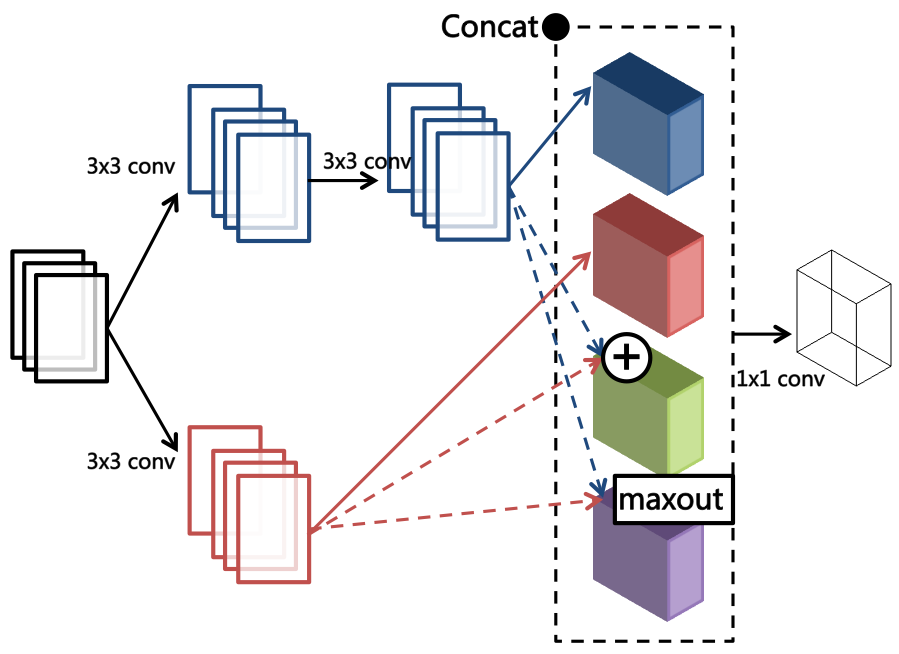
\includegraphics[width=1.0\linewidth]{sam_arc.png}
\caption{SAM结构。}
\label{fig:sam}
\end{figure}

结合盗梦空间结构Inception,最大化输出单元Maxout,残差网络ResNet,网络中的网络NIN这四个网络结构各自的特点与优势,本节设计并实现了一种组合卷积结构:自适应模块SAM。SAM以盗梦空间结构Inception为计算框架,包括四条特征提取分支和一个特征选择器。如图~\ref{fig:sam}所示,四条分支中包括两条具有不同深度和感受野大小的卷积分支,一条Maxout分支,一条残差分支。SAM可以公式化表示如下:
\begin{eqnarray} \label{equ:sam}
f^{1} &=& W_{11}x+b_{11} \nonumber\\
f^{2} &=& W_{22}\sigma(BN(W_{21}x+b_{21}))+b_{22} \nonumber\\
f^{3} &=& f^{1}+f^{2} \nonumber\\
f^{4} &=& \max(f^1, f^2) \nonumber\\
f^{c} &=& {\sigma}(BN(f^1; f^2; f^3; f^4)) \nonumber\\
f_{SAM} &=& {\sigma}(BN(W_{s}f^{c}+b_{s}))
\end{eqnarray}
其中 $f^{1}$ 是第一条卷积分支,具有 $3\times3$ 的感受野和 1 的深度;$f^{2}$为第二条卷积分支,采用具有 $3\times3$ 感受野大小的两个卷积层的简单堆叠,$f^{2}$ 具有 $5\times5$ 的感受野和 2 的深度;$BN$ 代表批正则化(Batch Normalization,BN)~\cite{ioffe2015batch}操作;$f^{3}$ 是 $f^{1}$ 和 $f^{2}$ 的和,该分支是残差分支,通过线性映射矩阵 $W_{11}$ 将输入 $x$ 映射为 $f^{1}$ , $f^{1}$ 与 $f^{2}$ 具有相同的特征维度,将 $f^{1}$ 加到 $f_{2}$ 上,使 $f_{2}$ 去学习相对于输入 $x$ 的残差函数,该分支的存在可以有效地加快SAM网络的训练过程,使网络更容易收敛;$f^{4}$ 是 $f^{1}$ 和 $f^{2}$ 的Maxout输出,用于增强SAM结构的非线性特征拟合能力,提高SAM网络的识别能力;$f^{c}$ 是四条分支的并集;最后通过一个具有 $1\times1$ 感受野大小的卷积层对 $f^{c}$ 特征进行筛选与压缩。因此, $1\times1$ 的选择器可以增强SAM结构在局部感受野范围内的特征非线性表达能力,在一定程度上起到特征压缩,降低后续网络计算复杂度。

\subsection{SAM的分析与讨论}
\label{sec:sap:model:discuss}

SAM的设计以盗梦空间结构Inception为基础框架,使SAM采用分组的方式进行特征提取,在没有明显增加网络参数的情况下增强SAM的特征表达能力。事实上,Inception也具有四条分支,分别是具有 $1\times1$,$3\times3$ 和 $5\times5$ 感受野的三个卷积分支,和一个池化分支。换一个方式理解,Inception的优势可以组合不同感受野的卷积和池化特征,并且通过 $1\times1$ 的卷积进行特征压缩。我们将类似的思想扩展到四个更加复杂、计算量更小、拟合能力更强、也更容易收敛的另外4个分支中。SAM具有两条卷积分支,分别具有 $3\times3$ 和 $5\times5$ 的感受野,一条残差分支,和一条Maxout分支。SAM的特征选择器用于合并这四条分支的特征,同时进行特征压缩与选择。SAM去掉了原Inception结构中 $1\times1$ 的卷积分支和池化分支,在我们的实验中,这两条分支对最终结果的影响不大,但引入这两条分支会增加网络的额外计算负担。

ResNet可以加快深层网络的收敛速度,通过增加一条或多条从浅层到深层的跨层短连接,来构建残差学习框架。He等人~\cite{he2015deep}的研究结果表明,当网络层数增加时,网络的测试精度会趋于饱和甚至下降。残差模型可以有效地克服这个问题,并且可以通过增加网络的深度来提高网络的泛化能力。SAM通过引入一条残差分支来继承残差结构易收敛的优势。值得一提的是,SAM通过复用 $f^{1}$ 和 $f^{2}$ 分支的计算结果来降低参数规模与计算量。SAM复用 $W_{11}$ 作为输入数据的线性投影矩阵,复用 $W_{21}$ 和 $W_{21}$ 作为残差模型主干网络的卷积参数,如图~\ref{fig:sam_review}(b)所示。此外,SAM采用参数复用的方式,可以有效地防止网络过拟合。

Maxout常常与Dropout一起被当做是一种模型平均技术来使用,理论上Maxout可以逼近任意非线性凸函数。但是Maxout的采用了多个线性卷积操作,需要较大的参数数量和计算量。SAM引入了Maxout结构作为四条分支之一,为了克服Maxout参数规模和计算量较大的缺陷,SAM同样复用了 $f^{1}$ 和 $f^{2}$ 两条分支来降低模型的参数和计算复杂度。该分支的引入可以有效地提高SAM结构的非线性特征表达能力。

NIN主要用于提高局部感受野范围内的特征非线性表达能力,事实上,NIN等价于在输出特征后面增加一或多个具有 $1{\times}1$ 感受野大小的卷积层。这样的结构在SAM中同样起到十分关键的作用。首先,$1\times1$ 的卷积结构同样可以增强局部感受野范围内特征的非线性表达能力。其次,SAM的选择器可以对输出特征进行维度上的压缩,从而减小网络运行时内存消耗与计算负荷。此外,该结构起到特征选择的作用,通过监督学习的方式,合理分配各特征的权重。

实际上,SAM并不局限于仅仅包含这四条分支,更多优秀的卷积网络分支有待加入SAM结构,对SAM进行改进与性能提升。

\section{实验结果}
\label{sec:sap:experiment}

在深度学习开源项目caffe~\cite{jia2014caffe}的基础上,我们实现了组合卷积SAM结构,并对SAM网络进行了对比实验。所有的实验均以数据并行的方式运行于具有2颗GPU核心的NVIDIA K80上。我们在四个图像识别数据集CIFAR-10~\cite{krizhevsky2009learning},CIFAR-100~\cite{krizhevsky2009learning},MNIST~\cite{lecun1998gradient}和SVHN~\cite{netzer2011reading}对SAM进行了测试实验。

\subsection{网络结构}
\label{sec:sap:experiment:arc}

\begin{figure}[t]
\centering
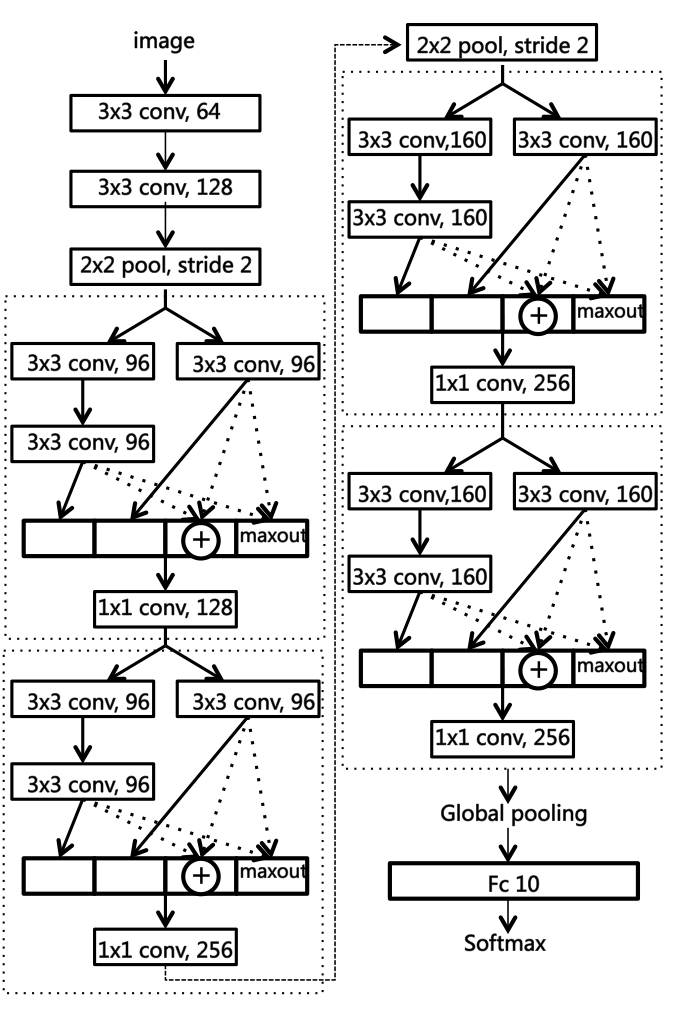
\includegraphics[width=0.8\linewidth]{sam_net.png}
\caption{SAM-Net:网络整体结构。}
\label{fig:net}
\end{figure}

本章所使用的网络结构如图~\ref{fig:net}所示,该网络包含了两个卷积层,四个SAM层,三个均值池化层和一个softmax层。

通常来说,卷积神经网络的初始阶段主要用于提取图像的低级特征,传统的卷积层已经具备很好的低层特征提取能力,并且可以节省大量的计算开销。因此,SAMNet的初始阶段采用两个传统的卷积层,用于图像底层特征的提取,之后是一个均值池化层。接下来,SAMNet采用两个SAM卷积层组成了网络的中间阶段,经过第二个均值池化层,另外两个SAM层组成了SAMNet的最后一个阶段。输入图像经过以上两个卷积层和四个SAM层所生成的特征连接到了一个全局池化层,最后通过Softmax对物体的概率进行预测。此外,批规划化BN和Dropout作用于每个卷积层之后,用于提高网络的泛化能力。

\subsection{网络参数}
\label{sec:sap:experiment:param}

\begin{figure}[!h]
\centering
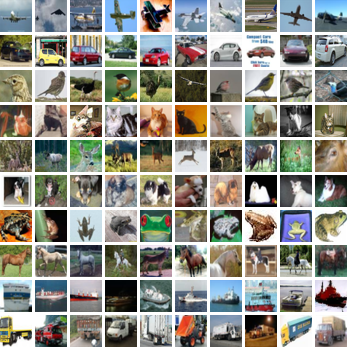
\includegraphics[width=1\linewidth]{sam_cifar10.png}
\caption{CIFAR-10测试样本示例。}
\label{fig:sam_cifar10}
\end{figure}


在所有的实验中,我们均采用批大小(batch size)为96的随机梯度下降(Stochastic Gradient Descent,SGD)算法来训练SAMNet。网络的初始学习率为 0.01,在训练过程中,每当损失函数达到局部极值而停止下降时,学习率被降低为原来的 $1/10$。持续减小学习率三次,直到学习率降低至 1e-5。在卷积层,卷积偏置的学习率是卷积核的 2 倍。训练过程中,采用 0.9 的动量因子(Momentum)来保证随机梯度下降算法的快速稳定。所有的参数均采用 0.004 的权重衰减(Weight Decay )。丢弃率为 0.1 的Dropout被用于除了第一层卷积之外的每个卷积层之前。对于四个数据集,我们均采用了相同的数据预处理,在训练数据集上计算出所有图像对应位置的BGR像素均值,记为均值图像,网络的输入图像是原始图像与均值图像的差。与~\cite{goodfellow2013maxout}不同,我们并没有对输入图像进行归一化或白化等其他额外预处理操作。

\subsection{CIFAR-10}
\label{sec:sap:experiment:cifar10}

我们首先从CIFAR-10~\cite{krizhevsky2009learning}数据集开始实验,Cifar是加拿大政府牵头投资的一个科研项目研究所,而CIFAR-10是Hinton的两个学生Alex Krizhevsky和Ilya Sutskever整理收集的一个物体识别数据集。CIFAR-10的图像是八千万微图片(80 Million Tiny Images Dataset)的一个标注子集,一共包含 60,000 张 $32\times32$ 的彩色图片,平均分为完全互斥的 10 类,每类具有 6,000 张图片。整个数据集被分成 5 组训练样本和 1 组测试样本,每组具有 10,000 张图片,即一共有 50,000 张训练图片和 10,000 张测试图片。CIFAR-10一共包含10个类别,分别是飞机、汽车、鸟、猫、鹿、狗、青蛙、马、轮船、卡车,如图~\ref{fig:sam_cifar10}所示。图~\ref{fig:sam_cifar10}中一共包含十行,每行代表一个类别,每类列举了十张训练样本。因为原始图片仅仅具有 $32\times32$ 像素大小,因此显示略显模糊。

\begin{table}[h]
\caption{CIFAR-10数据集上与已知模型的对比试验。}
\label{tab:cifar10}
\centering
 \begin{minipage}[t]{0.8\textwidth} 
 \begin{tabularx}{\linewidth}{L{6cm}C{4cm}}
 \toprule[1.5pt]
%\begin{tabular}{L{6cm}C{4cm}}
{\heiti 模型} & {\heiti 测试错误率(\%)} \\
\midrule[1pt]
\multicolumn{2}{c}{\heiti 没有数据增广} \\
\hline
Maxout \cite{goodfellow2013maxout}  & 11.68 \\
Prob maxout~\cite{springenberg2013improving}  & 11.35 \\
NIN~\cite{DBLP:journals/corr/LinCY13}  & 10.41 \\
DSN~\cite{lee2014deeply} &9.69 \\
%RCNN-96~\cite{liang2015recurrent} & 0.67 M & 9.31 \\
%RCNN-128~\cite{liang2015recurrent} & 1.19 M & 8.98 \\
RCNN~\cite{liang2015recurrent} & 8.69 \\
ALL-CNN~\cite{springenberg2014striving} & 9.08 \\
DenseNet~\cite{huang2016densely} & \bf{5.19} \\
\hline
SAMNet & \bf{7.53 (7.53${\pm}$0.17)} \\
\midrule[1pt]
\multicolumn{2}{c}{\heiti 有数据增广} \\
\hline
Maxout~\cite{goodfellow2013maxout} & 9.38 \\
Prob maxout~\cite{springenberg2013improving} & 9.39 \\
dasNet~\cite{stollenga2014deep} & 9.22 \\
DropConnect~\cite{wan2013regularization} & 9.32 \\
NIN~\cite{DBLP:journals/corr/LinCY13} & 8.81 \\
DSN~\cite{lee2014deeply} & 7.97 \\
%RCNN-96~\cite{liang2015recurrent} & 0.67 M & 7.37 \\
%RCNN-128~\cite{liang2015recurrent} & 1.19 M & 7.24 \\
RCNN~\cite{liang2015recurrent} & 7.09 \\
Highway Network~\cite{srivastava2015training} & 7.54(7.72$\pm$0.16) \\
ALL-CNN~\cite{springenberg2014striving}  & 7.25 \\
%ResNet-20~\cite{he2015deep} & 0.27 M & 8.75 \\
%ResNet-32~\cite{he2015deep} & 0.46 M & 7.51 \\
%ResNet-44~\cite{he2015deep} & 0.66 M & 7.17 \\
%ResNet-56~\cite{he2015deep} & 0.85 M & 6.97 \\
ResNet~\cite{he2015deep} & 6.43 (6.61$\pm$0.16) \\
%ResNet-1202~\cite{he2015deep} & 19.4M & 7.93 \\
DenseNet~\cite{huang2016densely} & \bf{3.46} \\
\hline
SAMNet & \bf{5.76 (5.76$\pm$0.13)} \\
 \bottomrule[1.5pt]
%\end{tabular}
 \end{tabularx}
\end{minipage}
\end{table}


为了验证SAM结构的有效性,我们在没有进行数据増广的情况下对SAMNet进行了测试,并且将实验结果与已知模型进行了对比分析,实现结果如表~\ref{tab:cifar10}所示。因为网络参数的初始化采用的是高斯随机初始化,为了避免单次实验结果的偶然性,我们对SAMNet进行了六次实验测试,分别得到7.52\%,7.76\%,7.34\%,7.54\%,7.35\%和7.68\%的测试错误率,即SAMNet在CIFAR-10上取得了一个均值为7.53\%,标准差为0.17\%的测试错误率。由表~\ref{tab:cifar10}可以看出,SAMNet以1.16\%的优势超过了之前精度最好的递归卷积神经网络RCNN~\cite{liang2015recurrent},但是和2017年提出的DenseNet~\cite{huang2016densely}相比,有所不足。

\begin{figure}[!h]
\centering
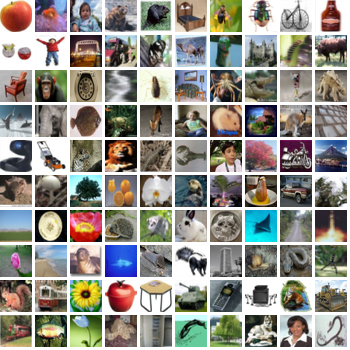
\includegraphics[width=1.0\linewidth]{sam_cifar100.png}
\caption{CIFAR-100测试样本示例。}
\label{fig:sam_cifar100}
\end{figure}


为了和之前的工作~\cite{goodfellow2013maxout,springenberg2013improving,stollenga2014deep,wan2013regularization,DBLP:journals/corr/LinCY13,lee2014deeply,liang2015recurrent,srivastava2015training,springenberg2014striving}保持一致,我们在有数据增广的情况下,对SAM-Net进行了实验测试。我们采用随机平移和图像水平翻转的数据增广方式,随机地从原始图像中截取 $24\times24$ 像素大小的图像样本,并随机对其进行水平翻转。在测试阶段,对每张测试图片,从图像的四角和中心位置截取出五张 $24\times24$ 像素大小的图像,并对这五张测试图像进行水平翻转,得到一共十张图像进行测试。最终的测试结果是这十张图像预测概率的平均值。我们同样进行了六次实验,分别得到5.98\%,5.82\%,5.70\%,5.67\%,5.78\%和5.63\%的测试错误率,最终得到了均值为 5.76\%,标准差为0.13\%的测试错误率。SAMNet的性能甚至超过了具有 100 层结构之深的ResNet~\cite{he2015deep}网络。通过多个SAM卷积模块的简单堆叠,SAMNet实现了复杂网络结构的识别性能,大大简化了网络的设计过程。



\subsection{CIFAR-100}
\label{sec:sap:experiment:cifar100}



CIFAR-100~\cite{krizhevsky2009learning}是一个与 CIFAR-10 类似的数据集,不同之处在于CIFAR-100具有 100 个物体类别。两个数据集具有相同的训练和测试图像规模,因此 CIFAR-100 中每个类别中图片数量只有CIFAR-10的 $1/10$。CIFAR-100的训练图像示例如图~\ref{fig:sam_cifar100} 所示,图~\ref{fig:sam_cifar100} 中包括 100 张图片,每张图片代表了 CIFAR-100 的一个物体类别,因为原始图像的分辨率较低,图像略显模糊。

\begin{table}[h]
\caption{CIFAR-100数据集上与已知模型的对比试验。}
\label{tab:cifar100}
\centering
\begin{tabular}{L{6cm}C{4cm}}
 \toprule[1.5pt]
{\heiti 模型} & {\heiti 测试错误率(\%)} \\
\midrule[1pt]
Maxout \cite{goodfellow2013maxout} & 38.57 \\
Prob maxout~\cite{springenberg2013improving}  & 38.14 \\
dasNet~\cite{stollenga2014deep}  & 33.78 \\
Tree based priors~\cite{srivastava2013discriminative} &  36.85 \\
NIN~\cite{DBLP:journals/corr/LinCY13} & 35.68 \\
DSN~\cite{lee2014deeply} & 34.57 \\
%RCNN-96~\cite{liang2015recurrent} & 0.67 M & 34.18 \\
%RCNN-128~\cite{liang2015recurrent} & 1.19 M & 32.59 \\
RCNN~\cite{liang2015recurrent} & 31.75 \\
ALL-CNN~\cite{springenberg2014striving}  & 33.71 \\
DenseNet~\cite{huang2016densely} & \bf{19.64} \\
\hline
SAMNet & \bf{28.56} \\
 \bottomrule[1.5pt]
\end{tabular}
\end{table}

在CIFAR-100数据集上,我们对本章提出的组合卷积网络SAMNet进行了测试,采用与第~\ref{sec:sap:experiment:arc}节相同的卷积神经网络结构,与第~\ref{sec:sap:experiment:param}节相同的网络参数设置,SAMNet在CIFAR-100上取得了28.56\%的测试错误率,实验结果如表~\ref{tab:cifar100} 所示。和其他网络结构相比,SAMNet的物体识别能力仅次于DenseNet,而在网络结构的设计上,采用组合卷积层搭建的SAMNet的设计更加简化与自由,且网络结构更具通用性。


尽管CIFAR-100与CIFAR-10具有相同的训练数据总量,但是类别的增加(增加十倍),单类别中图像样本数量的减少(减少十倍),增加了物体识别的难度。对于卷积神经网络来说,训练样本的数量对网络的识别能力具有重要的影响。训练样本数量的增加,有助于提高卷积神经网络的泛化能力。对于每个待识别的物体类别,卷积网络见过的图像越多,越有助于网络识别率的提高。从图~\ref{fig:sam_cifar10} 和图~\ref{fig:sam_cifar100} 可以看出,CIFAR-100和CIFAR-10具有十分相似的训练样本,但是CIFAR-100中单类别训练样本比CIFAR-10少了十倍(即一个数量级),导致CIFAR-100的测试错误率仅仅才达到28.56\%,与CIFAR-10数据集上7.53\%的测试错误率相比,高出了20多个百分点。


\subsection{MNIST}
\label{sec:sap:experiment:mnist}

\begin{figure}[!h]
\centering
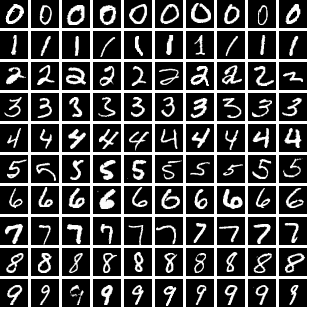
\includegraphics[width=1.0\linewidth]{sam_mnist.png}
\caption{MNIST测试样本示例。}
\label{fig:sam_mnist}
\end{figure}

MNIST~\cite{lecun1998gradient}是由阿拉伯数字 0-9 构成的手写体数字识别数据集,该数据集具有 60,000 张训练图像,10,000 张测试图像。每个手写体数字都被归一化居中显示在一个$28\times28$的灰度图像上,如图~\ref{fig:sam_mnist}所示。图~\ref{fig:sam_mnist}中一共包括十行,从上到下每行代表 0-9 的一个手写体类别,每一行列举了十张训练图像。

\begin{table}[h]
\caption{MNIST数据集上与已知模型的对比试验。}
\label{tab:mnist}
\centering
\begin{tabular}{L{6cm}C{4cm}}
 \toprule[1.5pt]
{\heiti 模型} & {\heiti 测试错误率(\%)} \\
\midrule[1pt]
Maxout \cite{goodfellow2013maxout}  & 0.45 \\
NIN~\cite{DBLP:journals/corr/LinCY13}  & 0.47 \\
DSN~\cite{lee2014deeply} & 0.39 \\
%RCNN-32~\cite{liang2015recurrent} & 0.08 M & 0.42 \\
%RCNN-64~\cite{liang2015recurrent} & 0.30 M & 0.32 \\
RCNN~\cite{liang2015recurrent} & \bf{0.31} \\
\hline
SAM-Net & \bf{0.31} \\
 \bottomrule[1.5pt]
\end{tabular}
\end{table}


相比于CIFAR-10与CIFAR-100的复杂彩色图像,MNIST数据集中手写体数字识别相对简单很多。使用与第~\ref{sec:sap:experiment:arc}节相同的卷积神经网络结构,与第~\ref{sec:sap:experiment:param}节相同的网络参数设置,SAMNet在MNIST数据集上取得了0.31\%的测试错误率,与递归卷积神经网络RCNN~\cite{liang2015recurrent}持平,如表~\ref{tab:mnist} 所示。组合卷积结构SAM,结合多个网络模型的优势,通过模型内多个复杂结构的有效组合,形成了一个通用的卷积神经网络模块,使用该模块可以有效地简化深层卷积神经网络模型的设计过程。尽管MNIST 与 CIFAR-10 和 CIFAR-100 具有不同的训练样本,但是使用组合卷积结构设计的卷积神经网络模型SAMNet,采用相同的网络结构,在多个不同的数据集上均取得了较好的识别能力。由此可见,组合卷积结构在不同数据集上具有较强的通用性。

\subsection{SVHN}
\label{sec:sap:experiment:svhn}

\begin{figure}[!h]
\centering
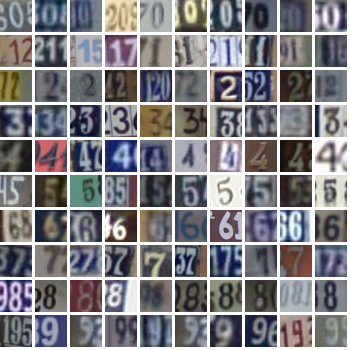
\includegraphics[width=1.0\linewidth]{sam_svhn.png}
\caption{SVHN测试样本示例。}
\label{fig:sam_svhn}
\end{figure}

SVHN~\cite{netzer2011reading}是一个采集自真实环境的图像数据集,其中的图片来自于谷歌街景中的房牌号。SVHN提供了两种格式的数据,这里我们采用第二种格式。该数据集包含了 73,257 张训练图像,26,032 张测试图像,和额外的 531,131 张相对比较简单的附加训练图像。SVHN数据集比MNIST更加复杂,识别难度也更大。因为SVHN的图片采集自真实环境,图片的亮度与光照变化较大。并且SVHN数据集的单张图像中可能会出现多个数字,这种情况,我们只识别中间位置的数字,如图~\ref{fig:sam_svhn}所示。图~\ref{fig:sam_svhn}中包括十行,从上到下每行代表一类样本,每类包含十张测试图像样本。

我们采用与Goodfellow~\cite{goodfellow2013maxout}类似的训练和测试步骤。从训练数据的每个类别中选取 400 张图像,从附加的简单训练样本中每个类别选取 200 张图像,合在一起作为验证集,用于调节网络的学习率与迭代次数。在SVHN数据集上,SAMNet取得了1.98\%的测试错误率,实验结果略差于RCNN~\cite{liang2015recurrent}和DenseNet~\cite{huang2016densely},如表~\ref{tab:svhn}所示。注意到递归卷积神经网络RCNN在四个数据集上采用相似的递归卷积结构,不同参数规模的网络对四个数据集进行的训练与测试。而本章所提出的由组合卷积结构搭建的卷积神经网络模型,在四个数据集上采用的是完全相同的网络结构和参数配置,具有更强的模型通用性。此外,本章提出的组合结构,不仅适用于本章提出的SAMNet,也可用于构建其他更宽更深的卷积神经网络结构,通过组合卷积的简单堆叠,来实现更复杂卷积网络结果的设计与优化。

\begin{table}[!h]
\caption{SVHN数据集上与已知模型的对比试验。.}
\label{tab:svhn}
\centering
\begin{tabular}{L{6cm}C{4cm}}
 \toprule[1.5pt]
{\heiti 模型} & {\heiti 测试错误率(\%)} \\
\midrule[1pt]
Maxout \cite{goodfellow2013maxout} & 2.47 \\
Prob maxout~\cite{springenberg2013improving} & 2.39 \\
NIN~\cite{DBLP:journals/corr/LinCY13} & 2.35 \\
DSN~\cite{lee2014deeply}  & 1.92  \\
RCNN~\cite{liang2015recurrent}  & 1.77 \\
DenseNet~\cite{huang2016densely} & \bf{1.59} \\
\hline
SAM-Net & \bf{1.98} \\
 \bottomrule[1.5pt]
\end{tabular}
\end{table}


\subsection{可视化}
\label{sec:sam:vis}

卷积神经网络在物体识别任务上取得了重大的研究突破,为了深入理解卷积神经网络的特征提取过程,本小结对卷积神经网络各卷积层特征进行了可视化与分析。

\begin{figure*}[h]
\centering
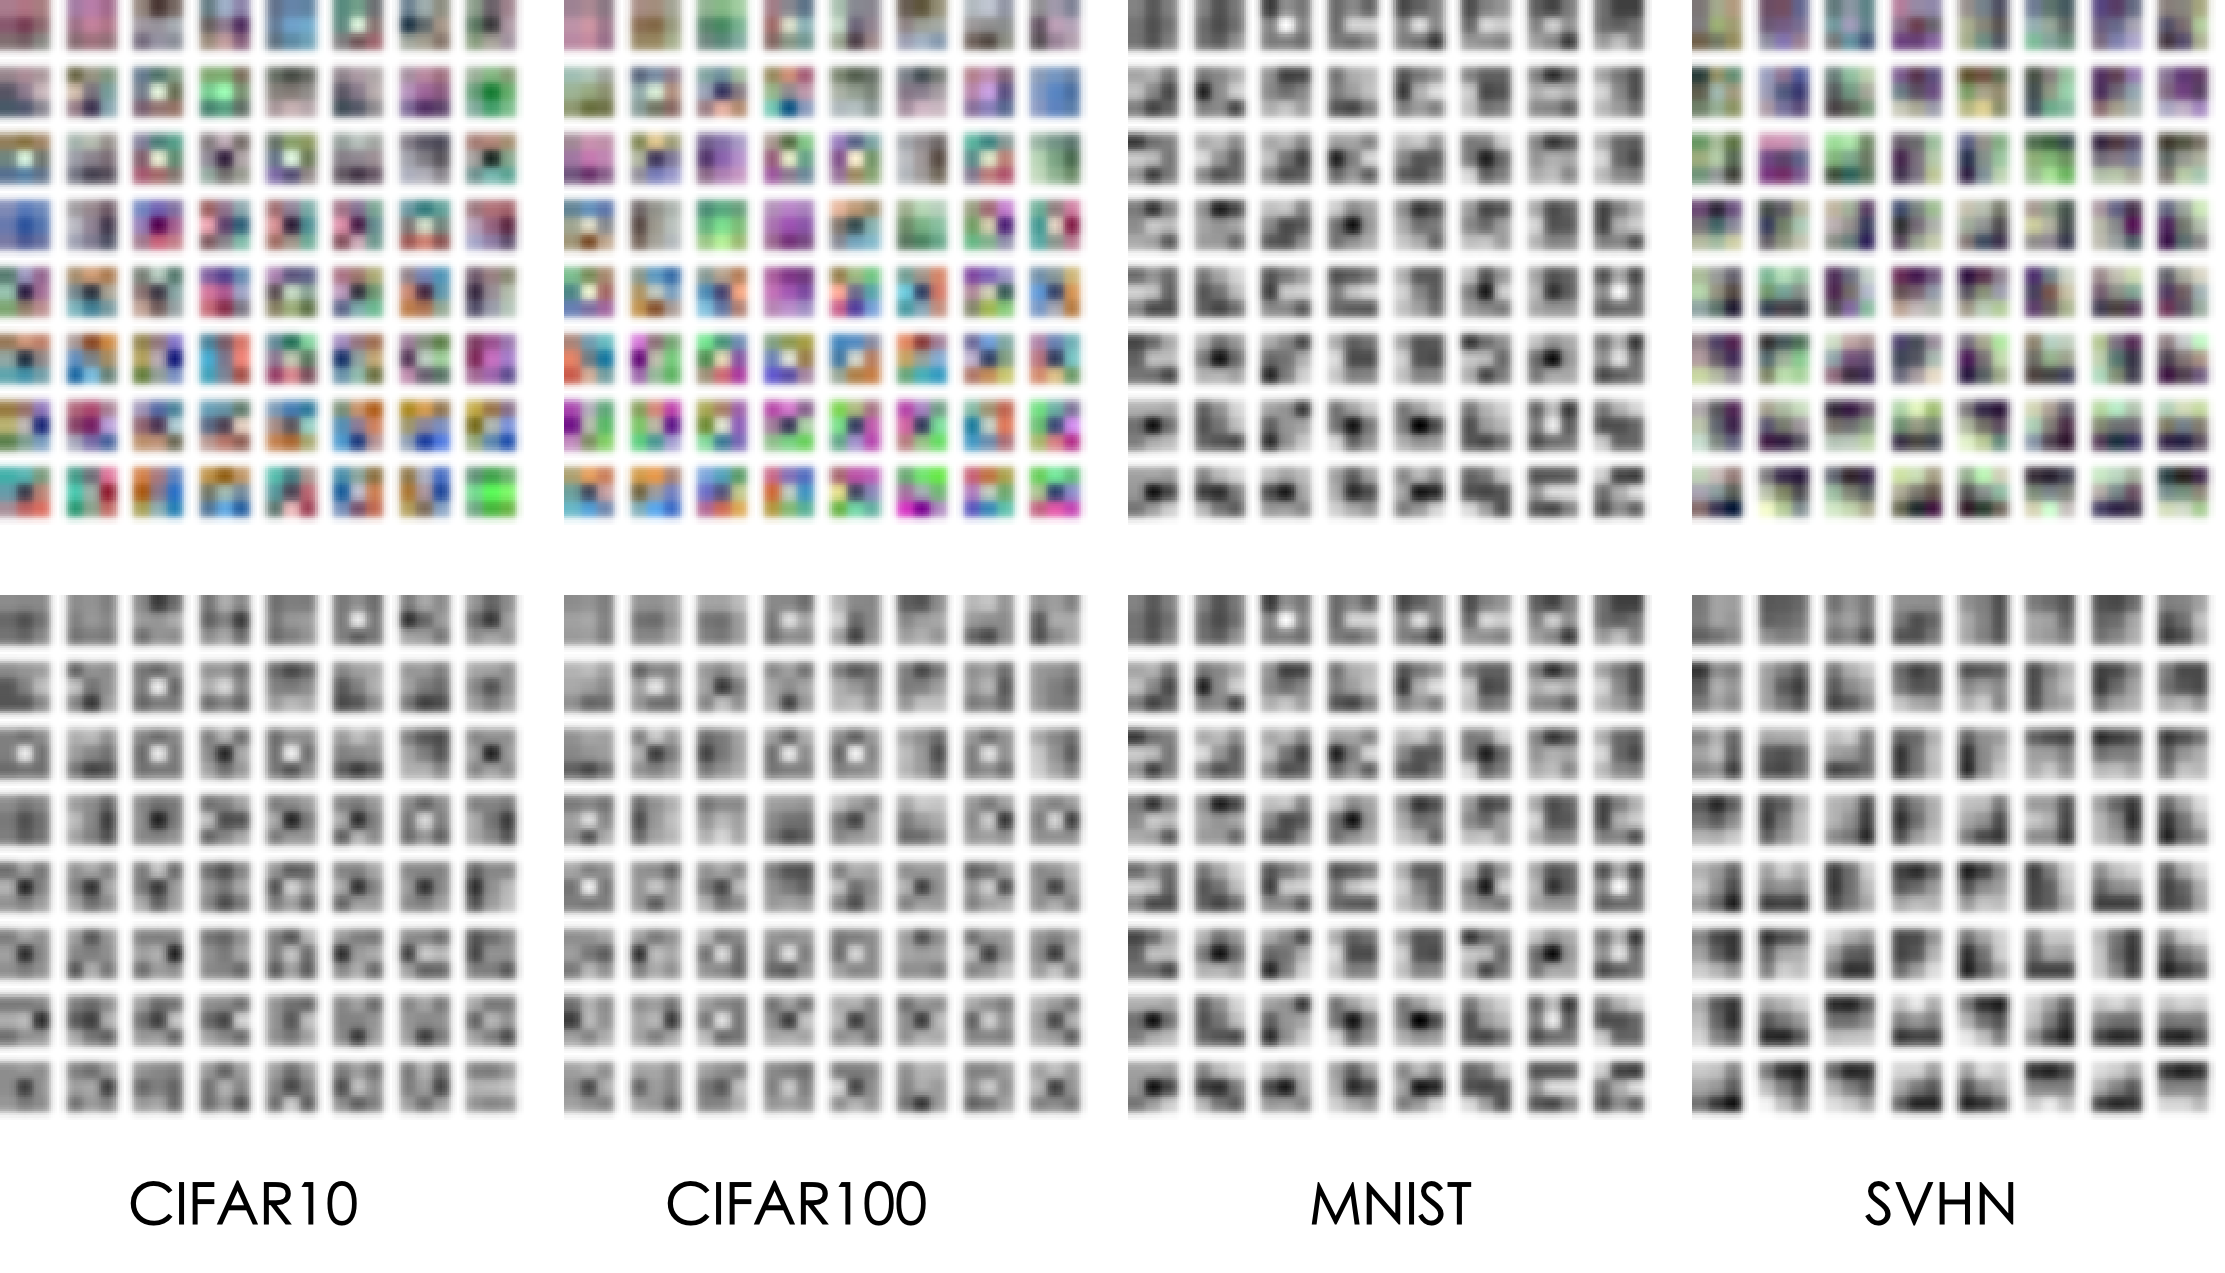
\includegraphics[width=1.0\linewidth]{sam_vis_filter.png}
\caption{第一层卷积核参数可视化。}
\label{fig:sam_vis_filter}
\end{figure*}

本节首先对卷积神经网络的浅层卷积核进行了可视化,如图~\ref{fig:sam_vis_filter}所示。当网络训练完成之后,通过将卷积核参数投影到图像空间,我们对第一个卷积层中64组卷积核参数进行了可视化。图~\ref{fig:sam_vis_filter}第一行彩色图是原始卷积核可视化结果,对于CIFAR-10、CIFAR-100和SVHN三个数据集,因为输入的图像为三通道彩色图像,因此对应的卷积核也具有三个通道,可以将卷积核参数投影到图像BGR颜色空间。但是对于MNIST数据集,原始的输入图像是单通道灰度图,对应的第一层卷积核只具有一个通道,只能投影成灰度图。为了将四个数据集上学习到的卷积参数进行对比,我们将四个数据集上训练得到的特征核图像均转换成灰度图,对应的实验结果如图~\ref{fig:sam_vis_filter}第二行所示。

从图~\ref{fig:sam_vis_filter}中可以看出,四个数据集上学习出的第一层卷积核参数具有很高的相似度。这是因为对于卷积神经网络的浅层来讲,学习到的往往是一些边缘信息。此外,从图~\ref{fig:sam_vis_filter}可以看出,CIFAR-10与CIFAR-100的卷积核相似度最高,MNIST和SVHN的卷积核相似度较高。由此可见,对于相似的识别任务,学习到的卷积核也更为相似。可见,对于不同类型物体的识别任务,卷积核学习到的特征也会有所差异。

本章提出了组合卷积结构用于简化复杂的深层卷积神经网络的设计过程,通过融合多个卷积模型的主要优势,提出了组合卷积结构SAM。SAM以Inception结构为基础计算框架,由四条特征提取分支与一个特征选择器组成,其中两条卷积分支具有不同的深度和感受野,一条残差分支用于加快SAM结构的收敛速度,一条Maxout分支用于提高SAM结构的非线性拟合能力。选择器具有特征压缩与选择的功能,增强网络局部感受野范围内的非线性拟合能力。为了更进一步理解SAM的特征提取过程,本章对SAMNet各个卷积层的隐层特征进行了可视化分析。


\begin{figure}[h]
  \centering%
  \begin{subfigure}{0.13\textwidth}
    
\includegraphics[width=1\linewidth]{sam_cifar10_in.png}
    \caption{输入图像。}
  \end{subfigure}%
  \hspace{1em}%
  \begin{subfigure}{0.8\textwidth}
    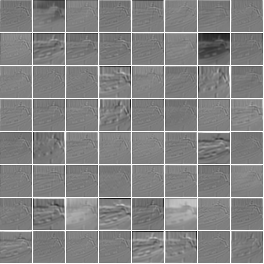
\includegraphics[width=1\linewidth]{sam_cifar10_conv1.png}
    \caption{第一个卷积层的输出特征图。}
  \end{subfigure}
  \caption{CIFAR-10数据集上,浅层卷积输出的特征图。}
  \label{fig:sam_cifar10_conv1}
\end{figure}


\begin{figure}[h]
  \centering%
  \begin{subfigure}{0.45\textwidth}
    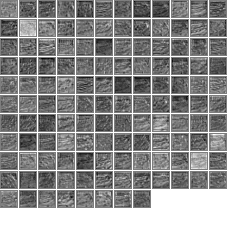
\includegraphics[width=1\linewidth]{sam_cifar10_conv2.png}
    \caption{第二个卷积层的输出特征图。}
  \end{subfigure}%
  \hspace{1em}%
  \begin{subfigure}{0.45\textwidth}
    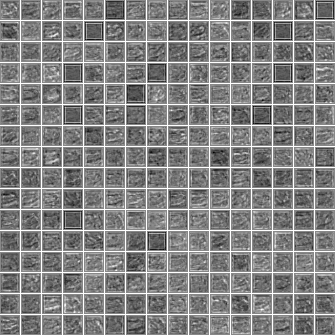
\includegraphics[width=1\linewidth]{sam_cifar10_conv3.png}
    \caption{第三个卷积层的输出特征图。}
  \end{subfigure}
  \caption{CIFAR-10数据集上,中层卷积输出的特征图。}
  \label{fig:sam_cifar10_conv3}
\end{figure}

\begin{figure}[h]
  \centering%
  \begin{subfigure}{0.45\textwidth}
    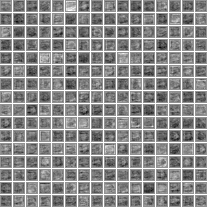
\includegraphics[width=1\linewidth]{sam_cifar10_conv4.png}
    \caption{第四个卷积层的输出特征图。}
  \end{subfigure}%
  \hspace{1em}%
  \begin{subfigure}{0.45\textwidth}
    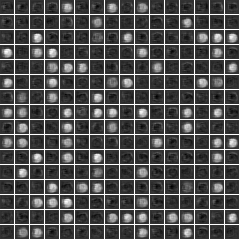
\includegraphics[width=1\linewidth]{sam_cifar10_conv5.png}
    \caption{第五个卷积层的输出特征图。}
  \end{subfigure}
  \caption{CIFAR-10数据集上,深层卷积输出的特征图。}
  \label{fig:sam_cifar10_conv5}
\end{figure}

在CIFAR-10数据集上,对于一张特定的输入图像,例如图~\ref{fig:sam_cifar10_conv1}(a)所示的轮船。本章对SAMNet网络的中间层卷积的隐层特征进行了可视化与分析,采用与卷积核参数可视化相似的投影方式,本章将各个卷积层的中间输出结果进行图像像素投影,得到的可视化结果如图~\ref{fig:sam_cifar10_conv1}、图~\ref{fig:sam_cifar10_conv3}和图~\ref{fig:sam_cifar10_conv5}所示,分别展示了SAMNet从第一层到第五层卷积的特征图可视化结果。SAMNet的网络结构如图~\ref{fig:sam}所示,一共包括五个卷积层,其中第一个卷积层为传统的卷积操作,其他四个为本章提出的组合卷积层。从图~\ref{fig:sam_cifar10_conv1}(b)可以看出,网络的浅层确实提取了图像的边缘和角点等低层特征,从图~\ref{fig:sam_cifar10_conv1}(b)的绝大部分特征图中都可以看出原始图像明显的边缘和角点特征。从图~\ref{fig:sam_cifar10_conv3}可以看出,网络的中层特征图相对来说更为复杂,从第二个卷积层的特征图可以看出,如图~\ref{fig:sam_cifar10_conv3}(a)所示,该层仍然在提取图像的边缘与角点信息,但是可以处理的图像感受野更大,学习到的特征更加鲁棒。网络的第三层特征图如图~\ref{fig:sam_cifar10_conv3}(b)所示,网络开始提取图像的一些纹理特征。从图~\ref{fig:sam_cifar10_conv5}可以看出,高层卷积层提取的特征与物体的类别更加相关,且具有更强的不变性。网络的第四层,如图~\ref{fig:sam_cifar10_conv5}(a)所示,图像的语义信息已经很难理解,但是其中高亮的部分往往表示了待识别物体的某些局部特征。网络的第五个卷积层的特征图具有更强的全局信息,可以很明显的从中看出待识别物体出现的大致区域,即图中高亮的部分。

\begin{figure*}
\centering
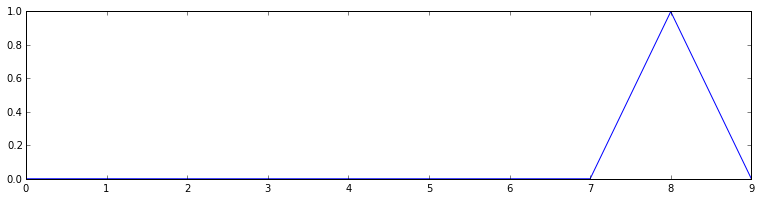
\includegraphics[width=1.0\linewidth]{sam_cifar10_out.png}
\caption{Softmax层各类别预测概率输出。}
\label{fig:sam_cifar10_out}
\end{figure*}

\begin{figure*}
\centering
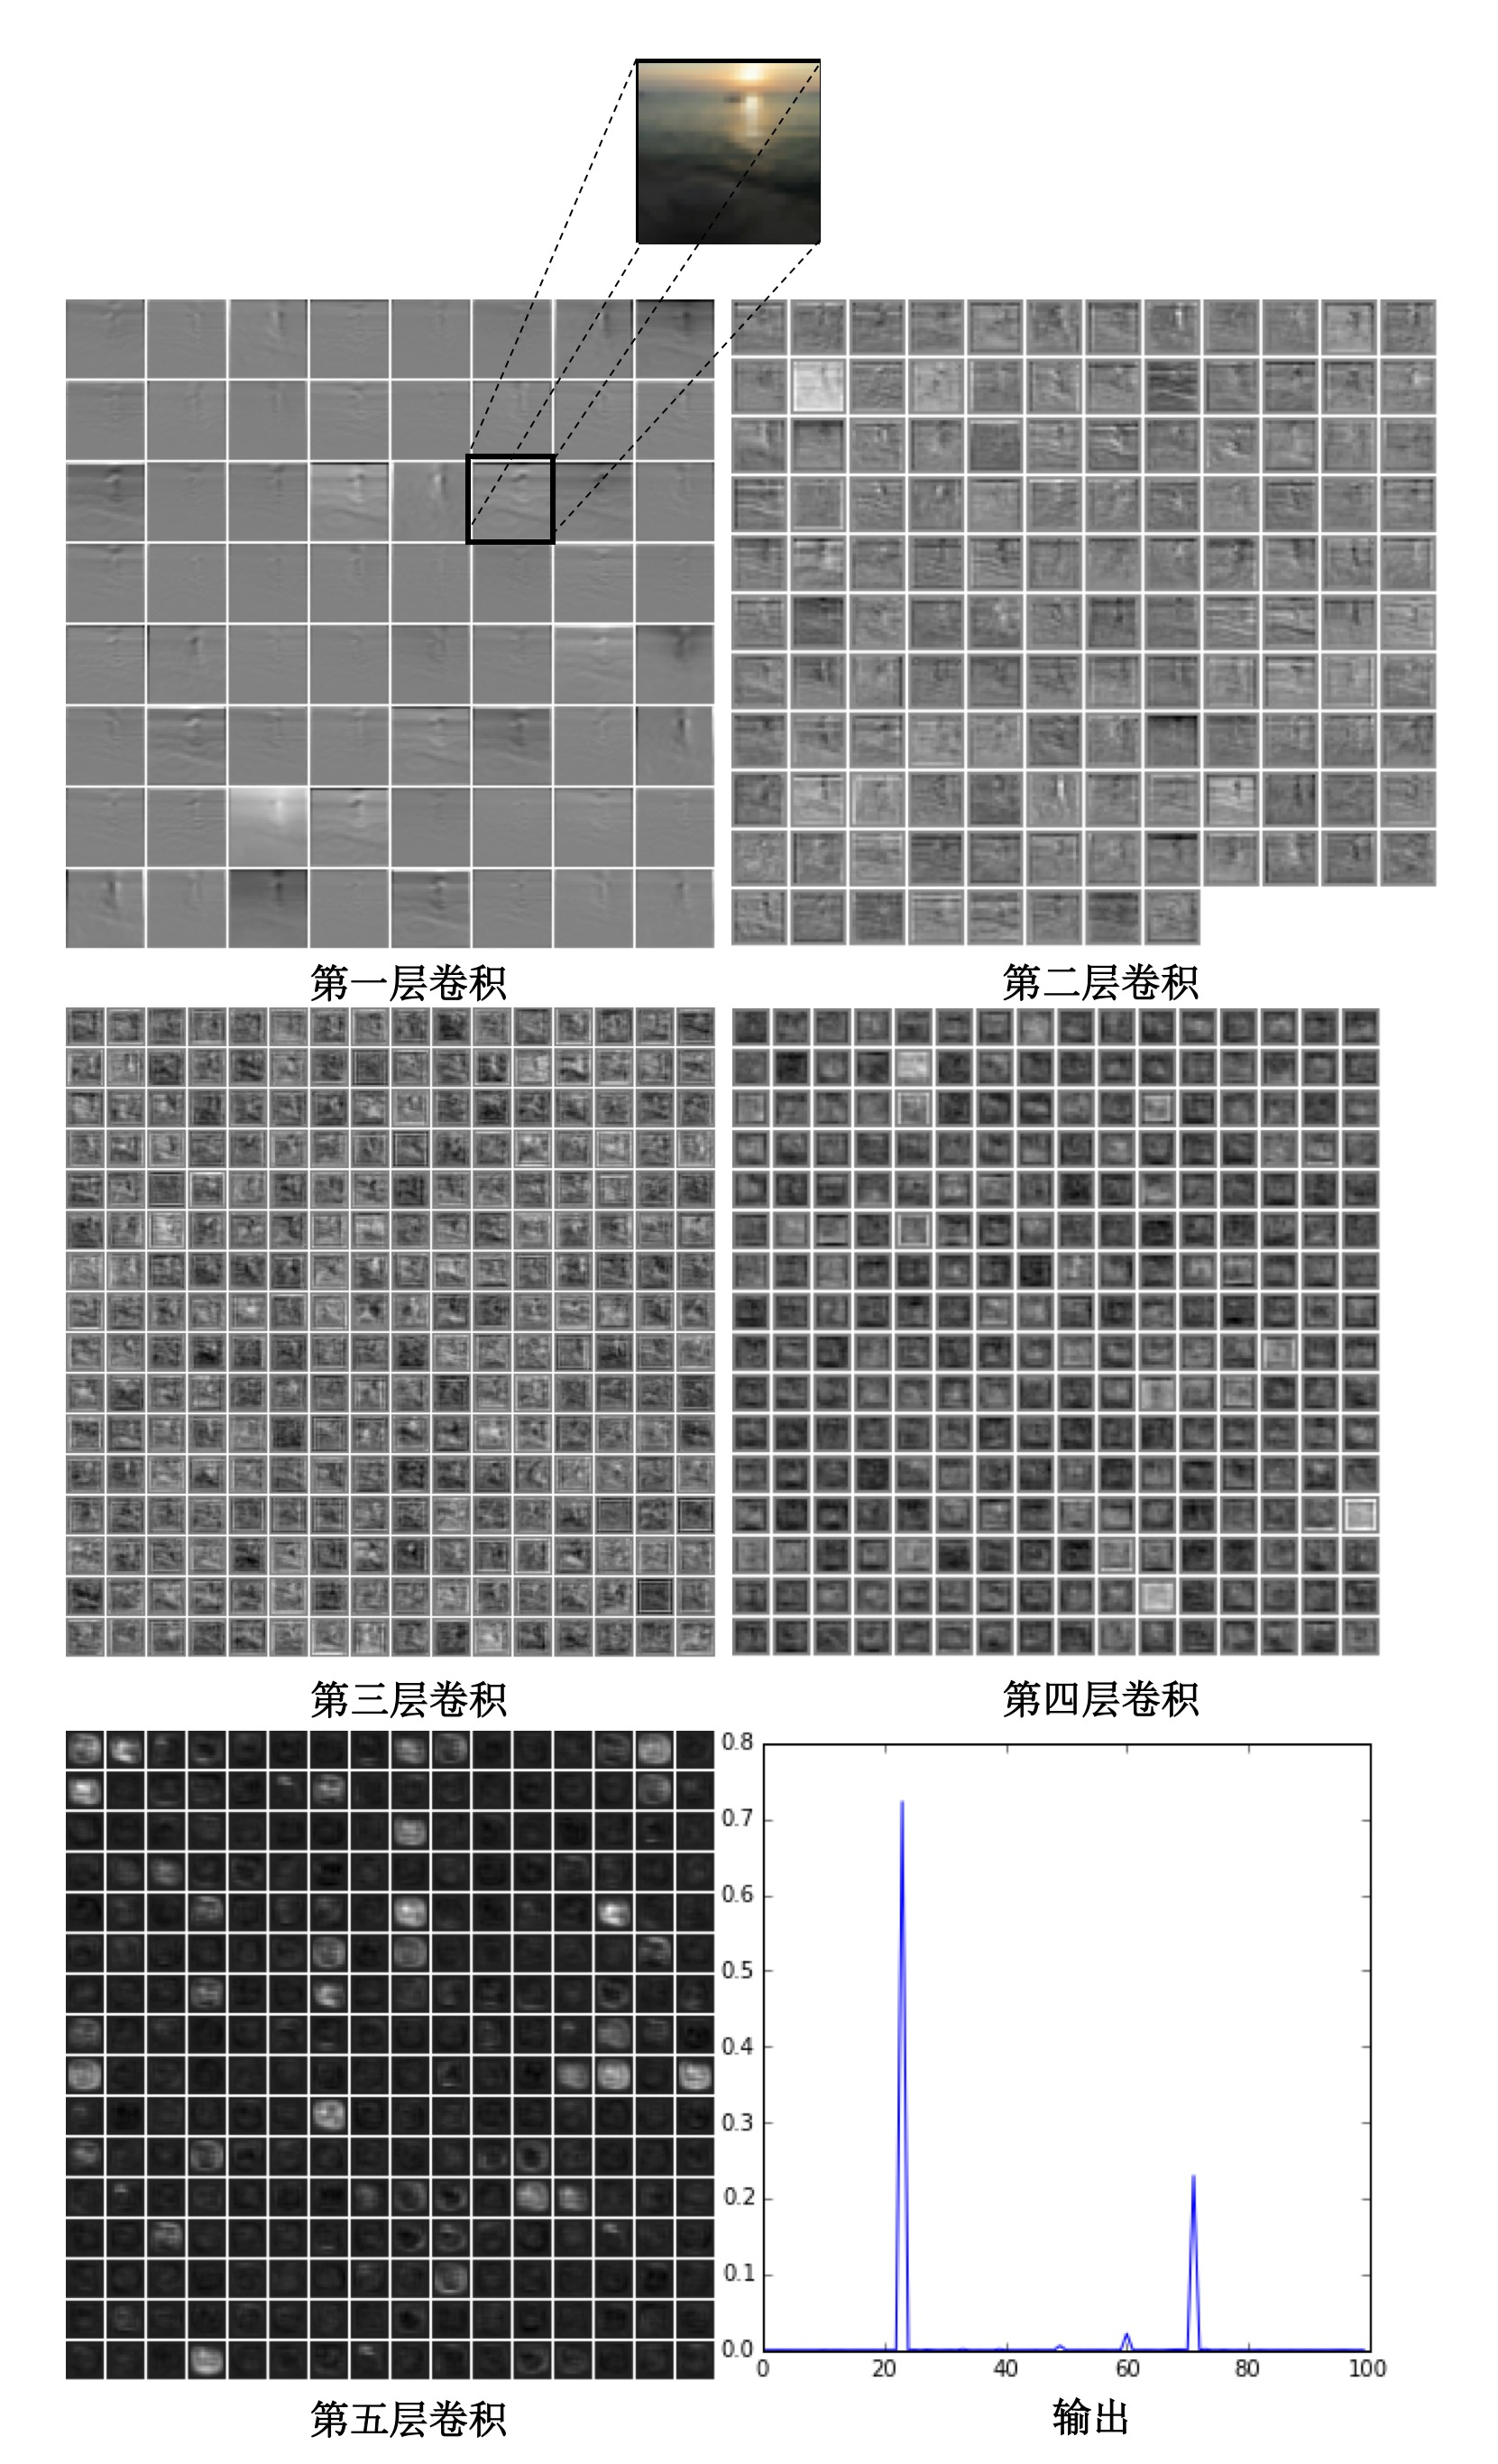
\includegraphics[width=1.0\linewidth]{sam_vis_cifar100.jpg}
\caption{CIFAR-100卷积层特征可视化。}
\label{fig:sam_vis_cifar100}
\end{figure*}

\begin{figure*}
\centering
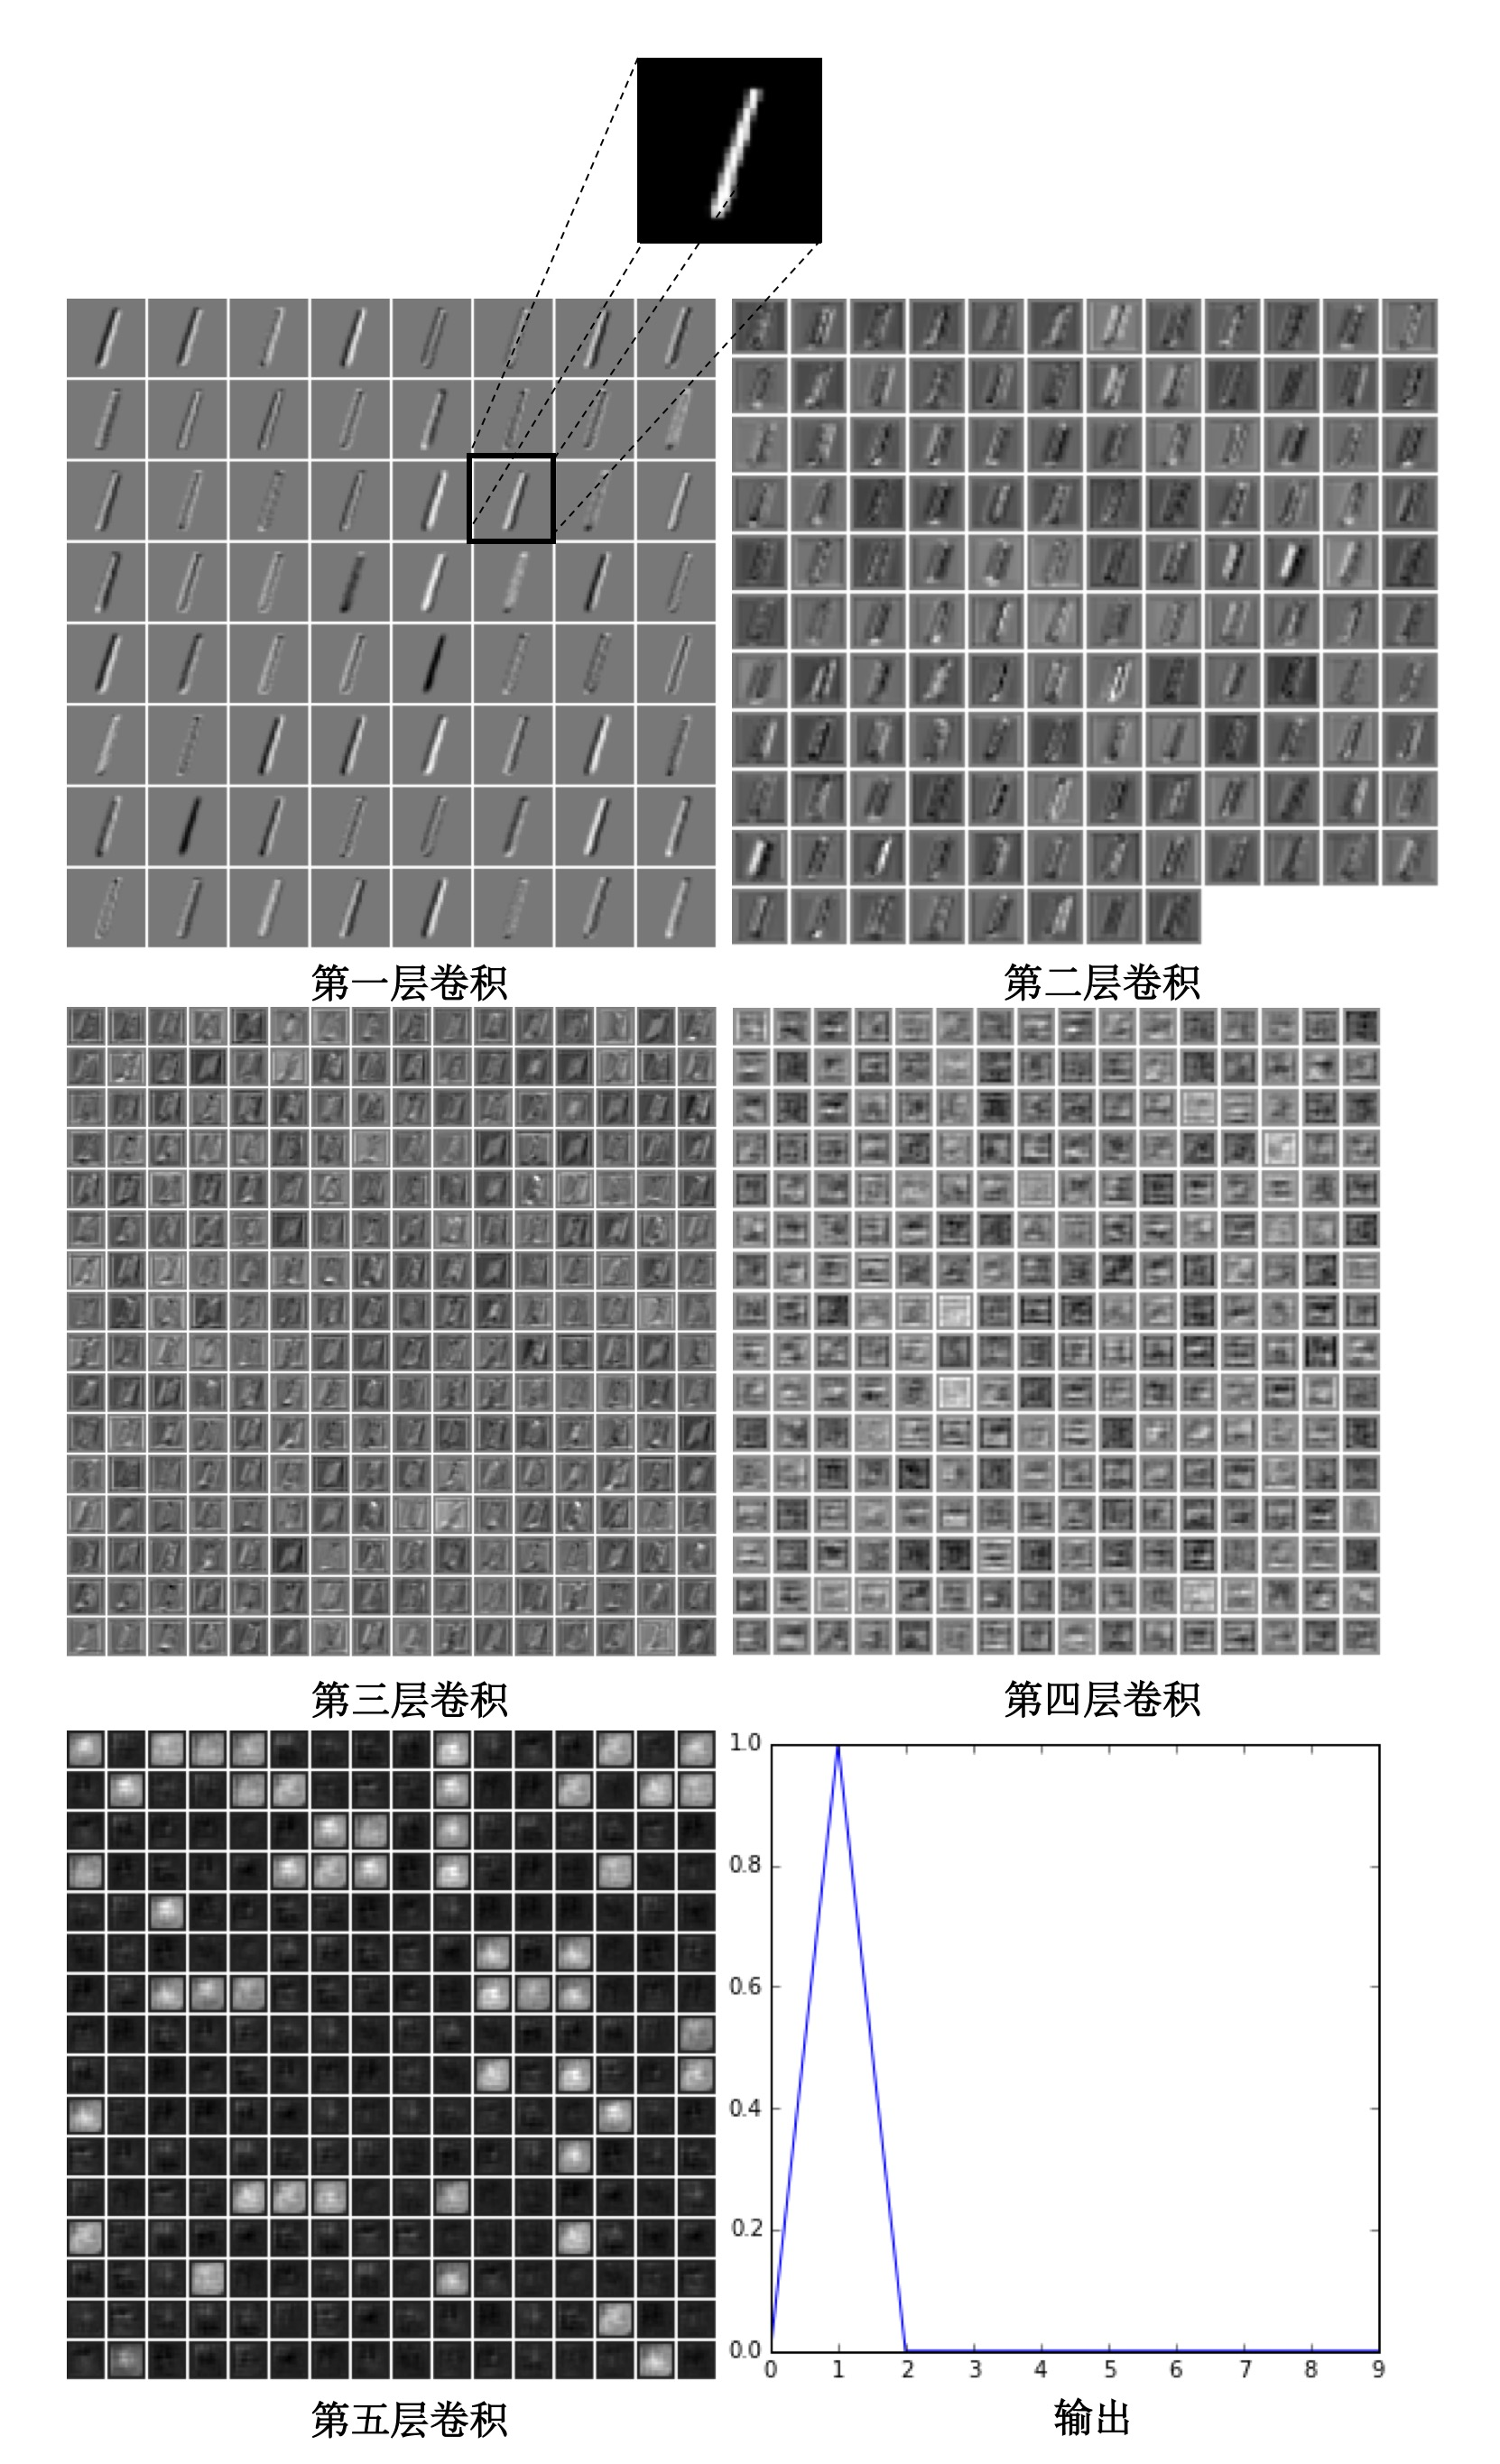
\includegraphics[width=1.0\linewidth]{sam_vis_mnist.jpg}
\caption{MNIST卷积层特征可视化。}
\label{fig:sam_vis_mnist}
\end{figure*}

\begin{figure*}
\centering
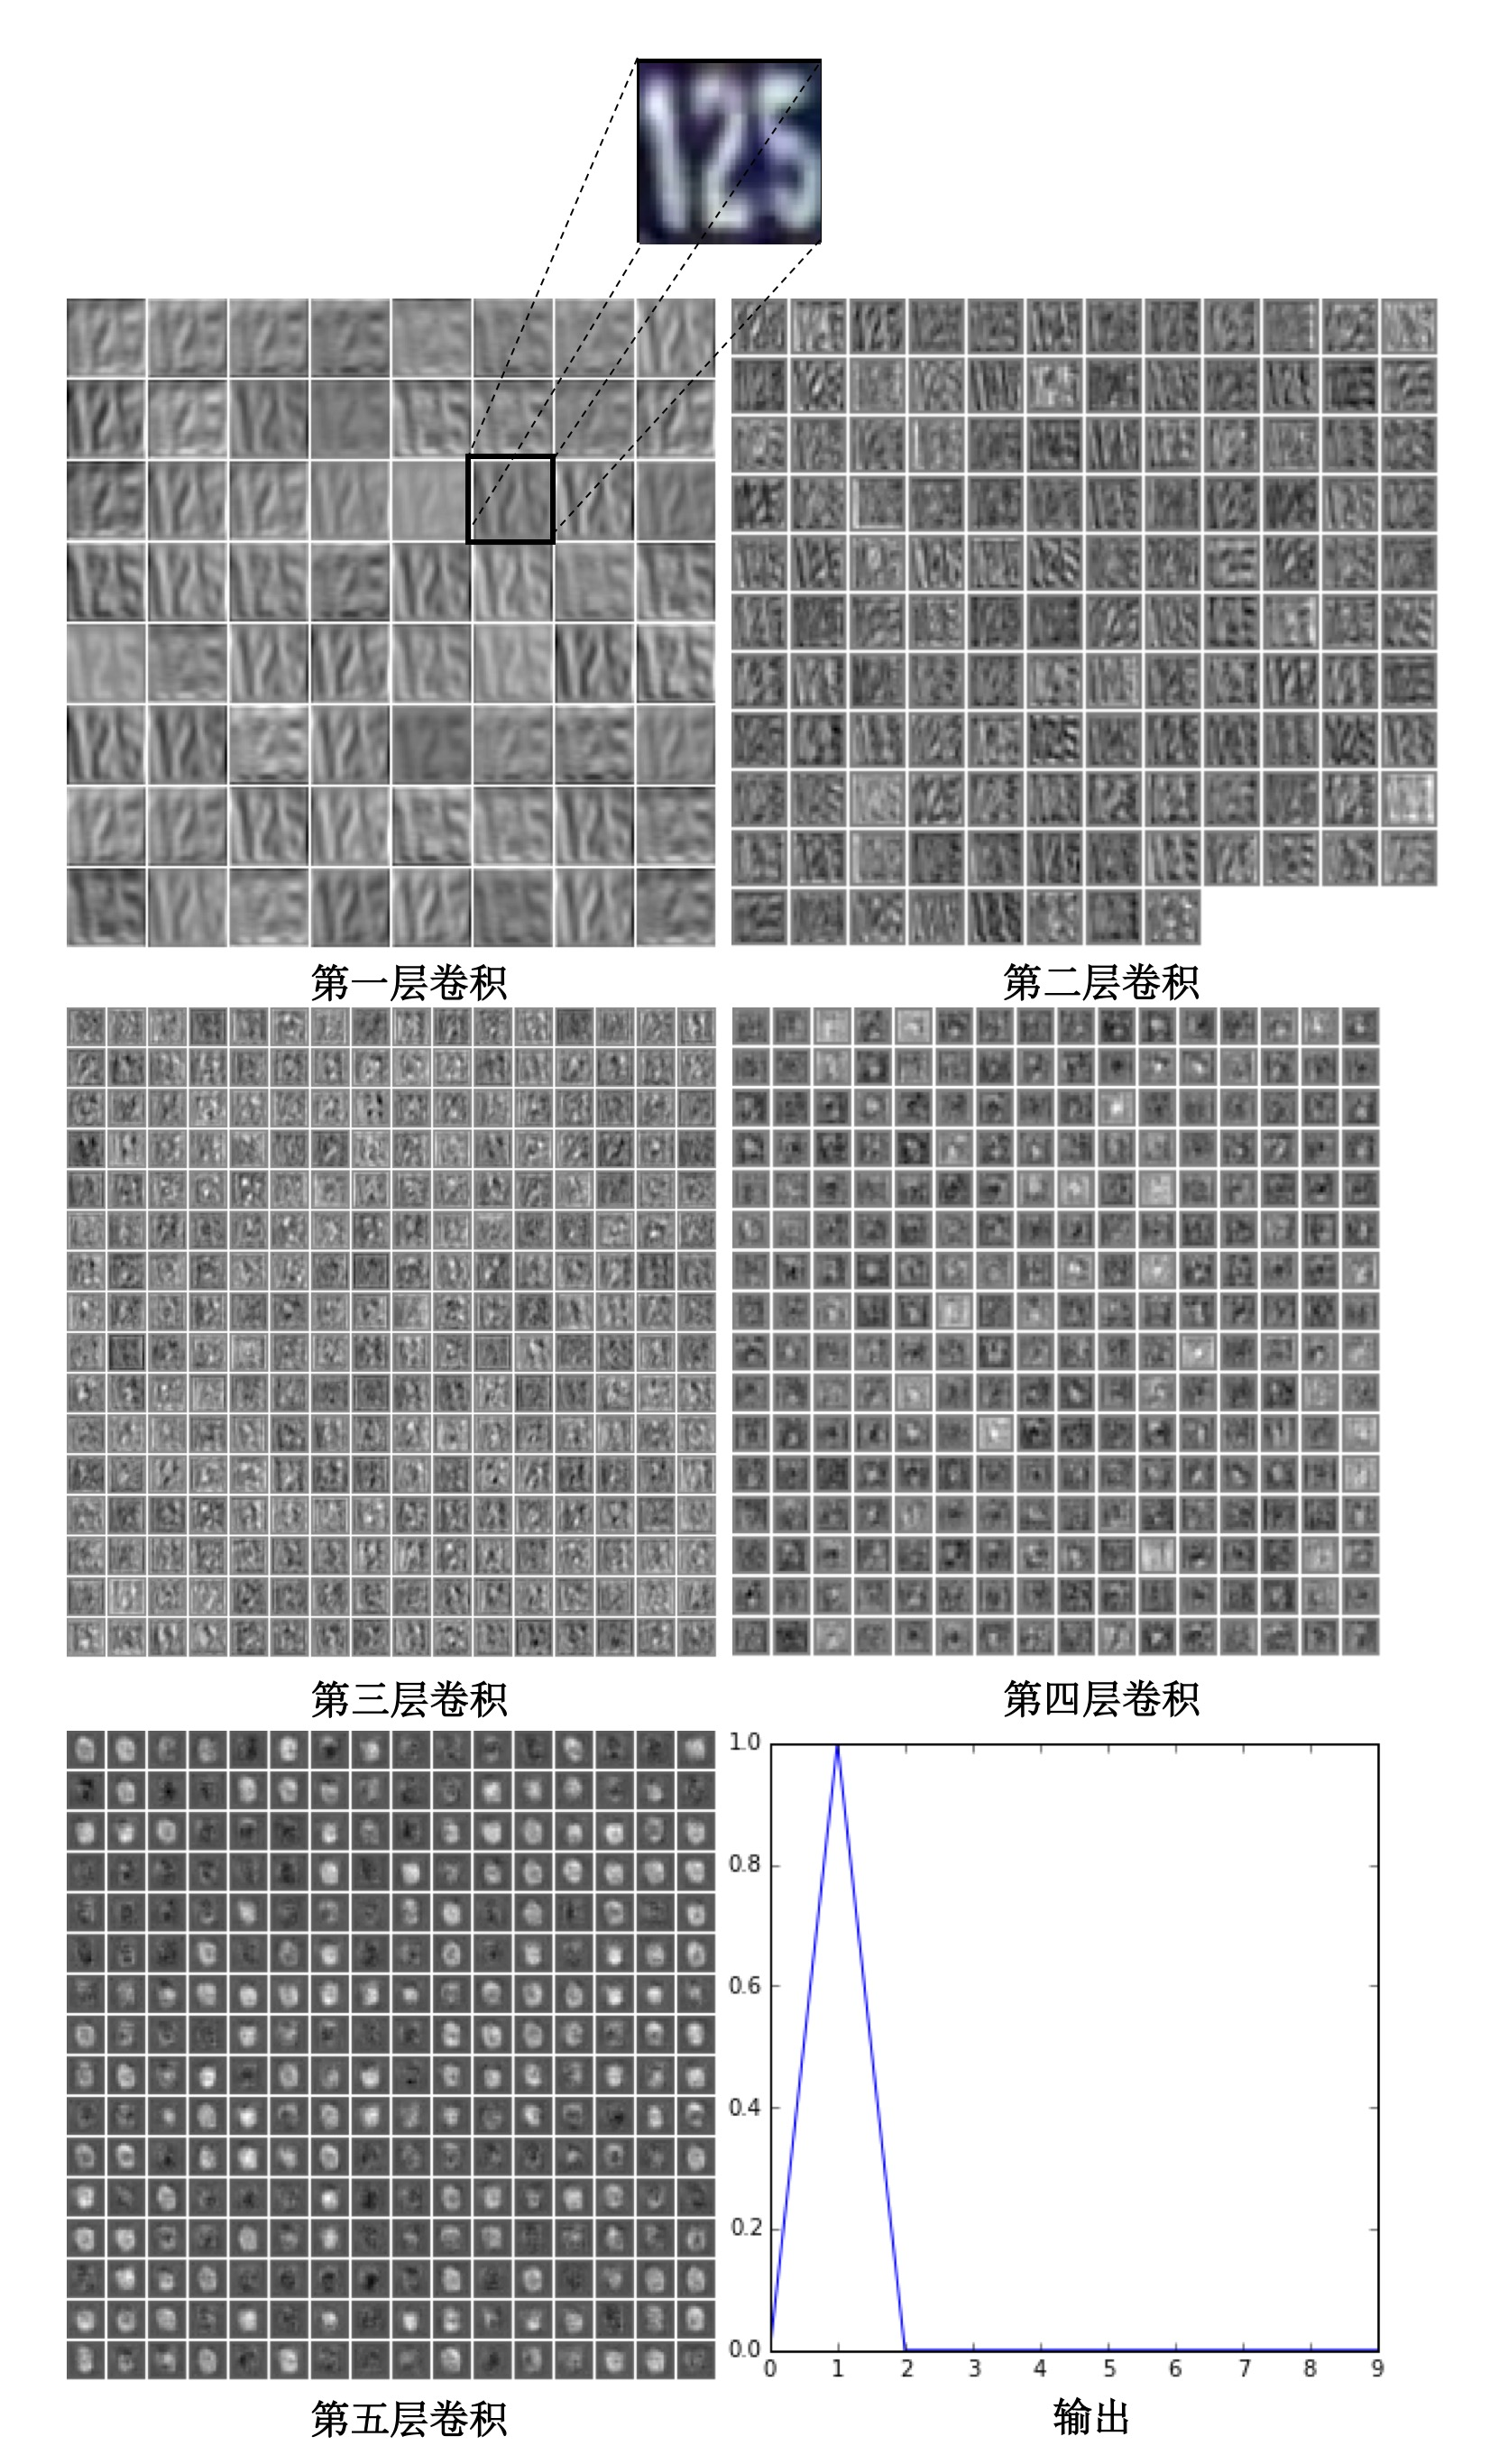
\includegraphics[width=1.0\linewidth]{sam_vis_svhn.jpg}
\caption{SVHN卷积层特征可视化。}
\label{fig:sam_vis_svhn}
\end{figure*}


卷积神经网络最后通过Softmax层来预测待识别图像的类别。对于CIFAR-10数据集这样的10分类问题,针对如图~\ref{fig:sam_cifar10_conv1}(a)所示的输入图像,SAMNet的Softmax层输出结果如图~\ref{fig:sam_cifar10_out}所示,SAMNet网络以0.9987的概率预测图~\ref{fig:sam_cifar10_conv1}(a)所属的类别是第8类(即轮船)。

为了增加上述可视化结果的可信度,我们在CIFAR-100、MNIST和SVHN三个数据集上均实现了上述可视化工作,实验结果如图~\ref{fig:sam_vis_cifar100}、图~\ref{fig:sam_vis_mnist}和图~\ref{fig:sam_vis_svhn}所示。其中对于CIFAR-100数据集,我们选了一个分类预测失败的例子,如图~\ref{fig:sam_vis_cifar100}所示。图~\ref{fig:sam_vis_cifar100}中输入样本是海滩,但是网络的预测结果却以0.7226的概率预测为第23类(青蛙)。尽管最终的分类结果有误,但是可以看出浅中层网络提取的特征仍然是图像的边缘与角点等低层特征,且较为清晰准确。此外我们发现,尽管网络最终的预测结果有误,但是网络仍然以一个较高的概率0.2296预测出物体也十分可能是海滩,即该图像的真实类别。可见即使是一个错误的预测概率,也具有很强的先验知识,第四章知识预回归方法即利用了这样的信息。


本章提出的SAMNet可以成功的应用于四个不同的图像识别数据集,其中组合卷积结构起到了十分重要的作用。对于相同的网络模型,针对不同的输入数据形式,组合卷积结构采用端到端学习的方式,可以优化得到适用于不同识别任务的特征提取方式,使得SAMNet网络可以在不改变网络结构的基础上,在四个数据集上均取得较好的网络泛化能力。


\section{本章小结}
\label{sec:sap:conclusion}

通过有效地结合Inception、Maxout、ResNet和NIN四个网络模型结构,本章提出了一种组合卷积结构:自适应卷积模块,用于简化复杂深层卷积网络的设计过程。SAM以Inception结构为基础计算框架,使SAM可以有效地平衡特征表达能力与网络的计算复杂度。SAM主要由四条特征提取分支与一个特征选择器组成,其中两条卷积分支具有不同的深度和感受野,一条残差分支用于加快SAM结构的收敛速度,一条Maxout分支用于提高SAM结构的非线性特征拟合能力。特征选择器具有特征压缩与选择的功能,还可以用于增强局部感受野范围内的非线性拟合能力。在CIFAR-10、CIFAR-100、MNIST和SVHN四个数据集上,SAMNet分别取得了5.76\%,28.56\%,0.31\%和1.98\%的测试错误率。实验结果表明,使用SAM模块组建卷积神经网络,可以大大简化深层卷积神经网络的设计,同时保持卓越的网络识别和泛化能力。















